\section{Proposed Approach}
\label{sec:proposed-approach}

Our goal is to visualize distributed state in a comprehensive way to
provide developers with an intuition about faulty behaviour. In order
to capture distributed state through variable logging, and the
aggregation of individual node state, we will leverage \dinv, a tool
for detecting likely data invariants in distributed
systems~\cite{dinv}. \dinv analyzes the logs of distributed systems, and computes the set of consistent cuts. Node states are grouped together by consistent cuts. The input to \dviz will be the partially ordered set of states computed by \dinv.

Distributed state is inherently complex. In its raw form it consists
of partially ordered instances of variable values. This raw data is
classically hard to reason about. To convey distributed state
to a developer it must be summarized. We propose that the state of
a distributed system under correct execution follows predicable
patters. Further that these patters are reflected the systems state.
The first contribution that our project seeks to make is a state
transition function $diff$ which measures the difference between
instances of distributed state. We recognize that many functions for
measuring state transitions could exist, our goal is to identify a general
$diff$ function which is sensitive to state transitions. An ideal $diff$ function would respond to state transitions predictably, and change minimally during repetitious behaviour.

Our initial approach will be to measure state transitions as the XOR
difference between variables in separate instances of distributed
state. We represent the state $\sigma$ of a system as a vector of
values $V = {v_1,v_2,\dots,v_n}$. The XOR difference between two
states $\sigma_i$ and $\sigma_j$ is $XOR(V_i,V_j)$. The resulting
vector contains an index for the XOR difference between each
variable value. The vector itself is $n$ dimensional and represents the XOR
difference of the systems state. The magnitude of this vector is the cange in distributed state. To measure the effectiveness of our
$diff$ function, we will initially plot its output as a simple line
graph and check if predictable repetitions patters emerge between
executions.  Furthermore, we plan to plot the first and second order
derivatives of $diff$, to determine
if they also exhibit predictable patters. Initially we will try to
detect patterns in toy systems. 


\begin{figure}[t]
    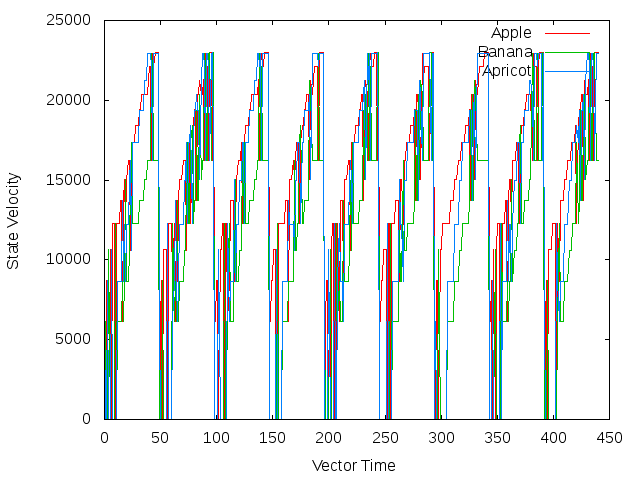
\includegraphics[width=0.50\textwidth]{fig/plot}
    \caption{\textbf{\dviz graph of a client-proxy-server interaction}}
\label{fig:plot} 
\end{figure}

To motivate the potential of the XOR function we constructed a prototype of \dviz. The prototype takes distributed state snapshots, derived by \dinv and outputs a line graph of each hosts state. Figure~\ref{fig:plot} was produced by graphing the states of 3 nodes configured as a client, a proxy, and a server which compute a linear formula. The value of all variable on each node were logged during the execution of the system, we made no attempt to track variable specific to the linear formula. We recognize that the prototype visualization is incomprehensible. However, there is a clearly visible correlation between the behaviour of the nodes, which repeats in a predictable pattern. Our initial findings suggest that XOR can be used to capture aspects of state transitions.

XOR may produce a predictable output, but it lacks a direct correlation to the developers understanding of the systems state transition. An alternative to XOR is to allow the user to specify a subset of variables, and encode the set of states they posses. For example, the user could specify that if a boolean variable \textit{leader} is true than a node is a leader of a Raft cluster, if false it is either a follower or a candidate. Transitions in the state's of variable can be modeled as distributed finite state automata, which have a large set of visual encodings~\cite{DBLP:journals/corr/abs-1110-4161}.


To visualize the transitional states, we need to first abstract the 
data and task, according to Munzner's nested model ~\cite{munzner2009nested}.
The original raw data to visualize can be regarded as a two dimensional 
spreadsheet, where each row represent a distributed state (variable),
 each column a snapshot and each cell the value of the variable at
 that particular snapshot.  The data type of the value is flexible,
 be it number, string, array or complicated dictionary.
However, there is little to do with this raw data if we do not derive
simplified data or transform it.  The way to do it actually depends on 
the transitional function we will experiment and concrete questions we
would like to answer with the visualization.  For example, if users want
to know the degree of change between snapshots, we can use the XOR function
to reduce each column (a vector of states at a snapshot) to a number,
whose difference is easily perceived when shown in a line chart.
It is yet early to talk about how kind of visual encoding to use before
we have a better understanding of the data and task.